% OMNIBOT PROPOSED -------------------------------------------------------------------------------------------------

\begin{figure}[!ht]

  \begin{subfigure}{0.5\textwidth}
  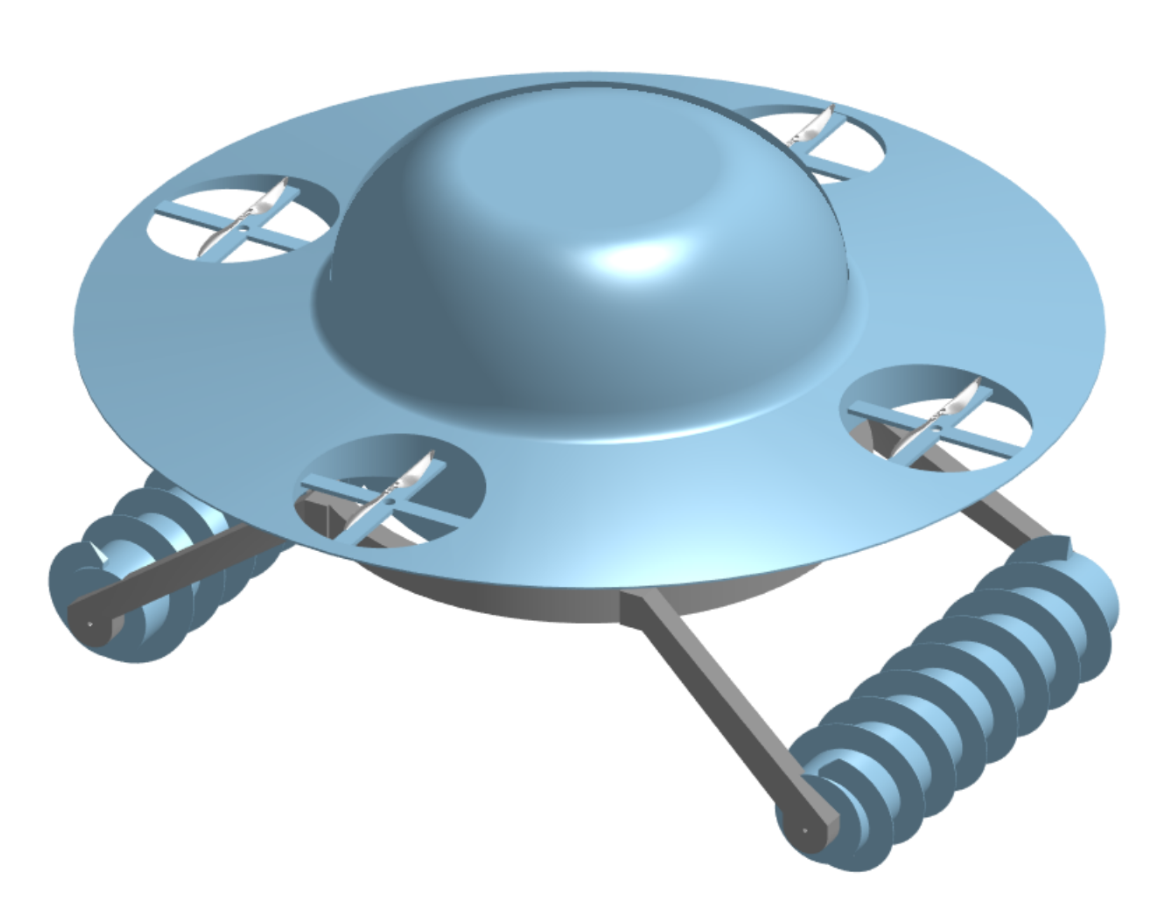
\includegraphics[width=\linewidth]{images/omnibot/omnibot_render_isometric.png}
  \caption{Omnibot Concept} 
  \label{fig:omnibot_render_iso}
  \end{subfigure}
  \begin{subfigure}{0.5\textwidth}
  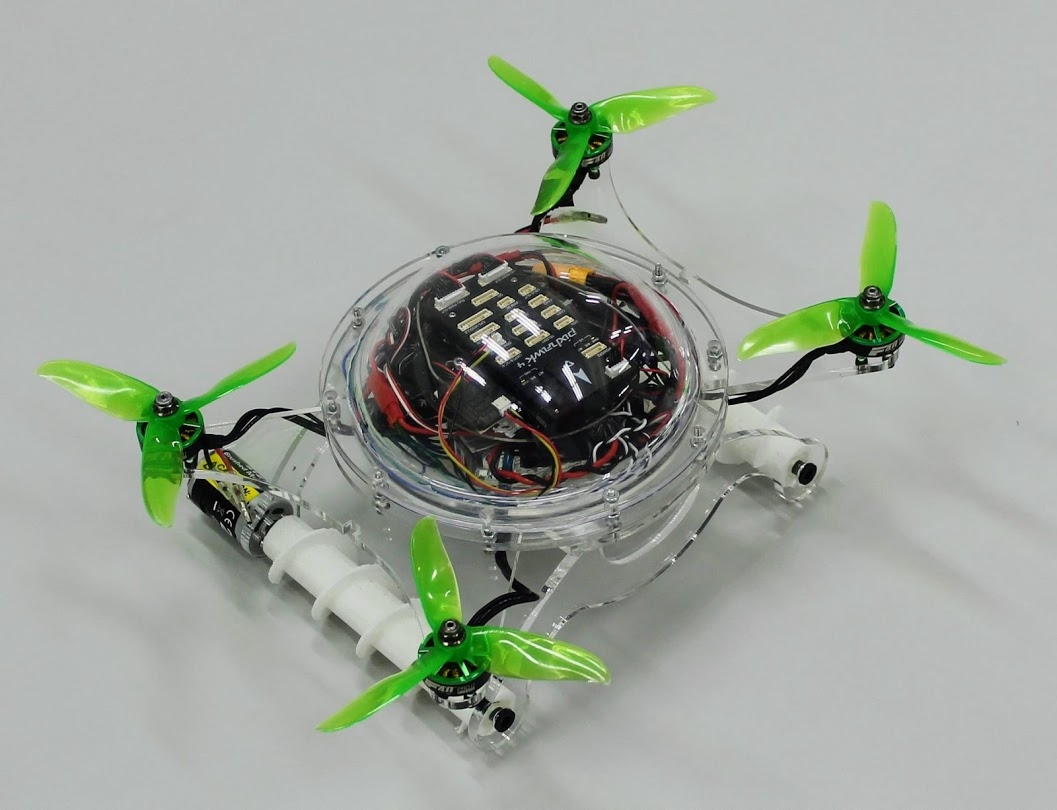
\includegraphics[width=\linewidth]{images/omnibot/omnibot_isometric.jpg}
  \caption{Omnibot Prototype} 
  \label{fig:omnibot_iso}
  \end{subfigure}
  
  \caption{Omnibot Design and Prototype}
  \label{fig:omnibot_prototype_design}

\end{figure}

The Omnibot is proposed as a multi-domain robotic platform for environmental monitoring capable of operating on land, in the air, and in the water. While there are robots capable of land-water, air-ground, and air-water locomotion separately, there is not a platform that performs in all three domains completely. The exception is the multi-field universal wheel for the air-land vehicle (MUWA)\cite{Kawasaki2013}. %Figure \ref{fig:muwa}.

The MUWA is a quad-copter that uses a variable pitch propeller scheme to direct the thrust from its four propellers to achieve VTOL and hover flight. On land, it is able to prop itself up on its outer structure, which consists of styrofoam rings, and function as a wheel, keeping itself upright via propeller thrust. It is also able to float on top of the water but is not capable of underwater navigation due to its permanently positively buyoant nature and construction. 

%\begin{figure}[!ht]
  %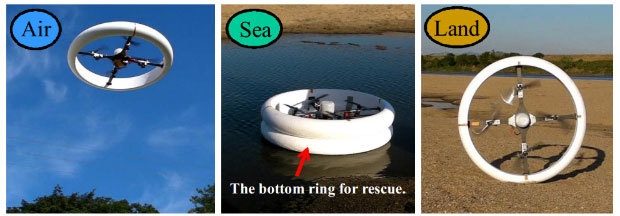
\includegraphics[width=\linewidth]{images/muwa.jpg}
  %\caption{The MUWA model (courtesy of \cite{Kawasaki2013})}
  %\label{fig:muwa}
%\end{figure}

To the author's knowledge, the Omnibot would be the first to navigate all three environments. The benefits would be numerous ranging from leveraging flight for faster travel or to overcome insurpassable obstacles, to landing for more precise measurements, to diving underwater for water quality monitoring, this versality is key to increasing capabilities in real world environments. 

\subsubsection{Prototype Design}

The proposed design will use a waterproof shell to house electronic components, a buoyancy control unit to dive and ascend in water, a dual screwdrive system for navigating land and water, a speed-control quad-rotor design for flight. A removable payload “disk” around its periphery would be used to extend the sensing capabilities of the robot while increasing the craft's aerodynamic properties. Payload disks could be configured with different sensors in order to allow easy deployment of many Omnibots with different capabilities. For example, one could have a payload for water quality measurements, while another could have a communications package and cameras. 

The Omnibot would utilize a NVIDIA Jetson board to simultaneously gather sensor data from a number of cameras pointing up, down, and around its body. This array of cameras would allow omnidirectional proprioception and leading to interesting opportunities for a number of activities such as: crop monitoring on land and air, lake health evaluation from the air, surface, and in the water, search and rescue missions, etc. 

To achieve these ambitious goals, an initial prototype will be built to study and optimize the robot around specific challenges inherent to operation in land, water, and air. Key design contraints are expected to be focused around achieving a weight, volume, and mass balance such that neutral buoyancy can be achieved, all while maintaining a sufficiently low weight to achieve flight within a feasible combination of commercial off the shelf battery, motors, and propellers. 

\begin{figure}[ht]

  \begin{subfigure}{0.5\textwidth}
  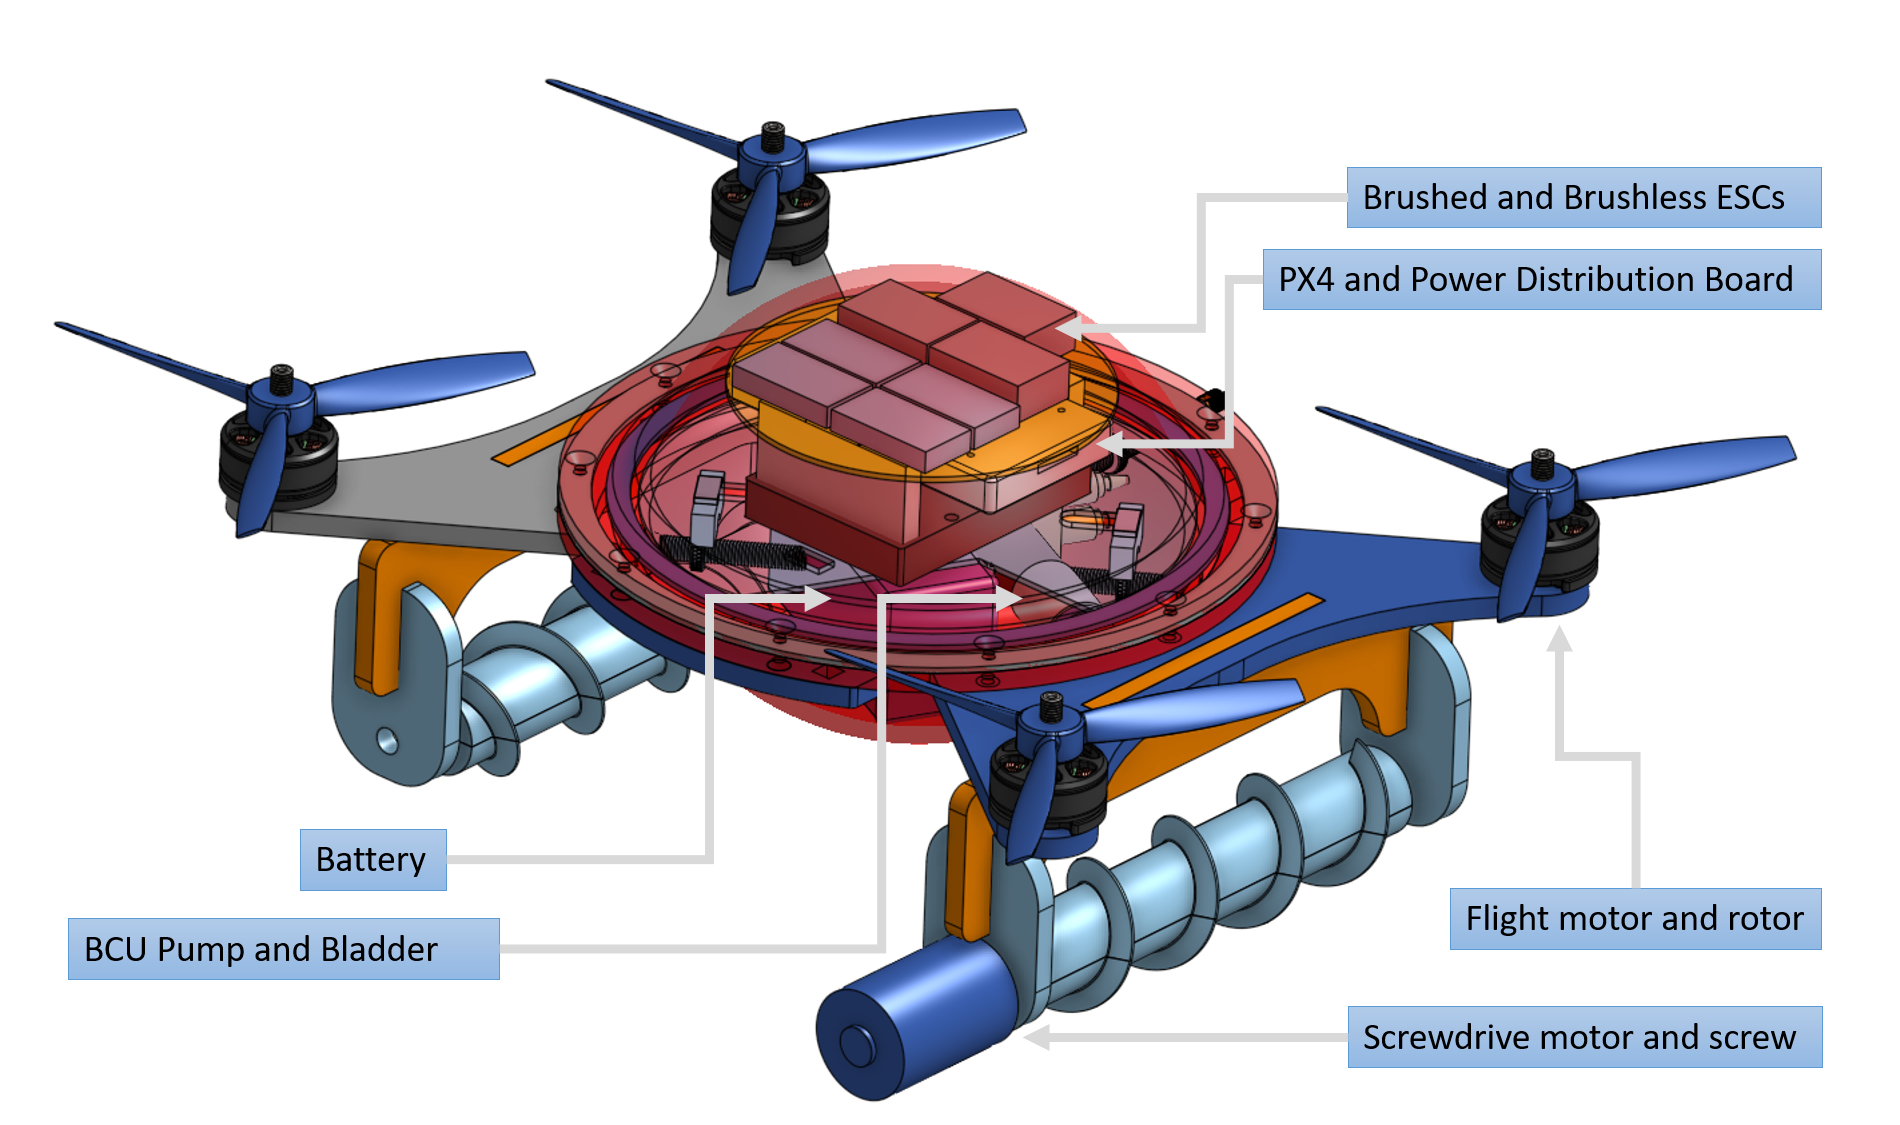
\includegraphics[width=\linewidth]{images/omnibot/omnibot_icuas_annotation.png}
  \caption{Omnibot Annotated Render} 
  \label{fig:omnibot_annotated_render}
  \end{subfigure}
  \begin{subfigure}{0.5\textwidth}
	\includegraphics[width=\columnwidth]{images/omnibot_electrical_schematic_tall.pdf}
  \caption{Omnibot Electronic System Schematic.}
	\label{fig:electronic_schematic} 
  \end{subfigure}

  \caption{Omnibot Design and Prototype}
  \label{fig:omnibot_electronics}

\end{figure}

Once the proof-of-concept prototype is built, the objective is to demonstrate navigation in all three domains as well as the transition between domains. Land-water, land-air, and water-air, as well as their reverse transitions are to be studied as these are expected to present their unique challenges, while being key to robust function. Once the prototype is successful, the next stage is to incorporate the environmental monitoring capabilities. This is expected to be accomplished via the integration of the sensor/payload disk on the periphery of the robot, as well as the integration of a high-level compute board, such as an NVIDIA Jetson board, for onboard processing. %The end result of these efforts would culminate a robot capable of carrying out environmental monitoring tasks in all three environments.  

%By leveraging a new propulsion method for land and water locomotion in conjunction with quad-rotor designs for flight, coupled with a waterproof hull and buoyancy control unit to alter its density, the Omnibot is able to travel on and through water, over land, and in the air. As far as we know, the Omnibot constitutes the first robot that could cover all four typical kinds of environments.

Covering all four mentioned domains presents a special challenge that is more than combining parts. As stated, there exist robotic solutions for each or a couple of domains, however, each has requirements or solutions that can be at odds with the requirements of a different domain. These challenges can be broken into the locomotive, structural, as well as electronic aspects, where locomotive covers the means by which the Omnibot is to move itself through a given media, structural covers the physical properties the platform has to deal with the four types of regions, and electronic is that which pertains to the power distribution, signal, and control of the robot. 
  
\subsubsection{Locomotion}

Central to the functionality and usability of a mobile robotic platform are the methods by which it moves itself through the environment it is in. Often, the aforementioned methods amount to be a fundamental choice as they place constraints on battery life, feasible paths to be followed, and the type of terrain to be traversed, variables which are of critical importance to all mobile platforms with a limited supply of power. 

A dual-parallel screw screwdrive powertrain was chosen for its ability to traverse both land and water environments as shown in Figure~\ref{fig:omnibot_iso}. It employs two independently actuated and contra-rotating continuous propellers. The screws consists of a cylinder with blades forming a helix around its surface. When rotated in a coordinated fashion, these allow a variety of movements. 

For flight, a quad-copter design was chosen based on its ability to provide the necessary amount of thrust, stability, and, most importantly, because vertical-take-off-and-lift (VTOL) allows effective air-ground and air-water transitions. Additionally, VTOL allows the robot to land carefully atop the screwdrive subsystem. When transitioning from water to air, the Omnibot was designed such that the propellers sit above water line. Fixed-wing alternatives would have placed additional and incompatible restrictions on weight, size, and other variables all while increasing the size. 

This design uses the T-Motor F40 Pro II KV2400 motors which weigh 29.5 grams a piece, yet are able to provide a theoretical 1400 grams of thrust when at full throttle and paired with a 4 cell Lithium Polymer battery. Additionally, underwater operation is achievable via a buoyancy control unit, as on the Aquapod. 

\subsubsection{Structural Design}

The majority of the Omnibot's electronic parts are enclosed within an transparent acrylic sphere, which is formed of two transparent hemispheres that clamp onto an O-ring that sits on a custom gland in one of the hemisphere's flanges.  The spherical design was chosen aero and hydrodynamic purposes and the transparency of the enclosure allows for cameras to be added inside without any further modifications.

The enclosure sphere is connected to the flight motors via a set of independent wings that are bolted to the sphere using the same bolting pattern that seals the two hemispheres. These motors are located at the extremities of the wings and are designed such that the DALPROP 4045 tri-blade propellers are sufficiently far away from the robot to avoid collision during flight, but also to allow simple access to the shell. 

The robot itself is suspended 1.1 inches by two screwdrive "legs" which are press fit and acrylic welded orthogonoal to the wings. The clearance is helpful for land navigation purposes. The motors that power the screws bolt on to the legs for ease of access and maintenance. 

A removable payload “disc” around the globe will be used in the future to extend the capabilities of the robot. Mounting different sensor suites to the exterior of the robot, will allow customizability of groups of Omnibots.

The Omnibot weighs approximately 1,418 grams dry and with an empty bladder and its volume is designed such that the robot is 25 grams over the neutral buoyancy point, therefore, within the bladder's water capacity. 

\subsubsection{Electronics and Software }

The prototype is built by integrating off-the-shelf and custom-designed components as seen in Fig.~\ref{fig:electronic_schematic}. At the heart of it all is the 4-cell lithium battery which powers the entire system. The Pixhawk 4 flight controller board \cite{pixhawkadmin_introducing_2018} connects to the GPS/Compass and external remote controller. During flight, it directs signals to the brushless flight motors through the F35A electronic speed controllers. The Pixhawk is also used to send WPM signals to the brushed motors that power the BCU pump as well as the two external brushed motors of the screwdrive system. 

The PX4 flight stack \cite{noauthor_open_nodate} and the Pixhawk 4 were chosen for their versatility and configurability. The PX4 firmware stack is modified to allow powering of the additional actuators but also to add and allow switching between different operational modes: land, water, or air.  

\subsubsection{Laboratory Experiments}
\label{omnibot_experiments_lab}

\begin{figure}[h!]
   \begin{subfigure}[t]{0.30\textwidth}
     \includegraphics[trim=0 40 0 40,clip,width=\textwidth]{images/omnibot/omnibot_lab.png}
     \caption{Land locomotion.}
     \label{fig:omnibot_indoor_land}
   \end{subfigure}
   \begin{subfigure}[t]{0.38\textwidth}
     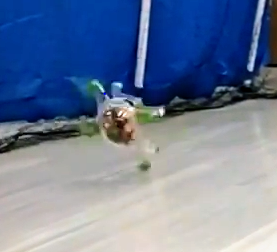
\includegraphics[trim=0 49 0 49,clip,width=\textwidth]{images/omnibot/omnibot_flip.png}
     \caption{Incipient flight.}
     \label{fig:omnibot_flip}
   \end{subfigure}
   \begin{subfigure}[t]{0.30\textwidth}
     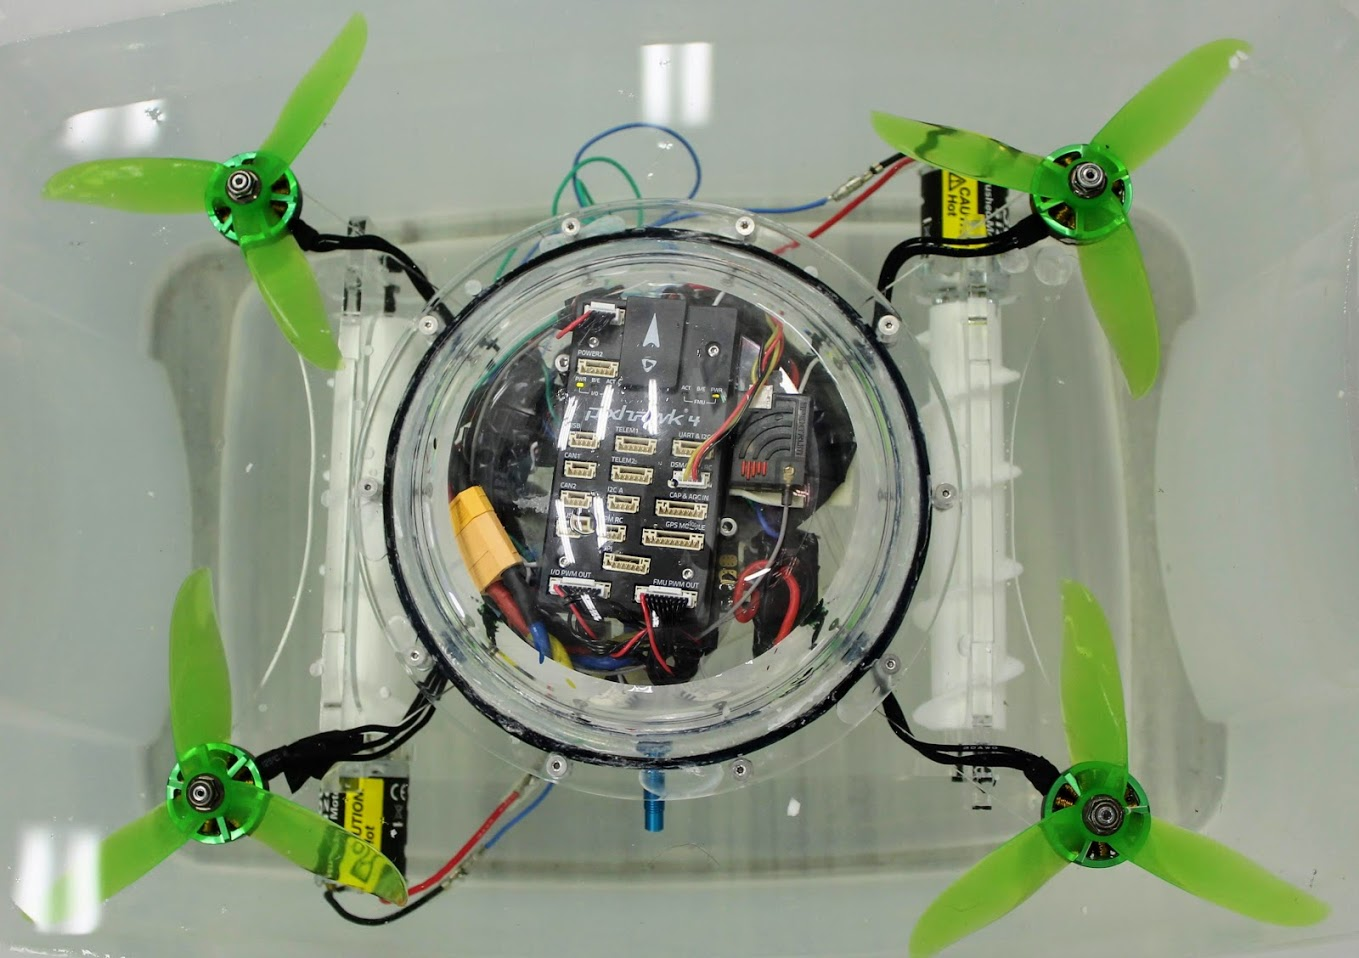
\includegraphics[width=\textwidth]{images/omnibot/omnibot_top.jpg}
     \caption{In water.}
     \label{fig:omnibot_lab_water}
   \end{subfigure}
   \caption{Indoor Omnibot prototype locomotion testing.}
   \label{fig:omnibot_lab}
\end{figure}


%The proof-of-concept model was first tested in each individual environment as shown in Figure ~\ref{fig:omnibot_lab}. 

The first tests involved testing the water-worthiness of the robot. The robot was subjected to bidirectional pressure gradients in order to stress test the main seal as well as the ports' seals. Internal pressure testing was done utilizing a compressed air line and visually verifying no air escaped while submerged in a container. The external pressure test was performed in a similar manner but with pressure provided by hydrostatic water pressure and visually inspecting for water within the clear shell, as can be seen in Fig.~\ref{fig:omnibot_lab_water}. 

Land locomotion was verified in a lab environment on relatively flat but roughly textured floors, as in Fig.~\ref{fig:omnibot_indoor_land}. The objective was to engage the screwdrive system and verify that the movement speed was controllable and adequate. As expected, in an impenetrable terrain of relatively high friction, the screws act like rollers with no tractive effort. 

Air function was verified within a controlled environment surrounded by a protective net. The goal here was to use the remote control to lift the robot off the ground. This test was successful in the Omnibot was able to create enough lift from its propulsion system to take-off from the ground. That being said, there is more work to be done in this area as control and weight balance was an issue. 


\subsubsection{Outdoor Experiments}
\label{omnibot_experiments_outdoor}

\begin{figure*}[h!]
   \begin{subfigure}[t]{0.30\textwidth}
     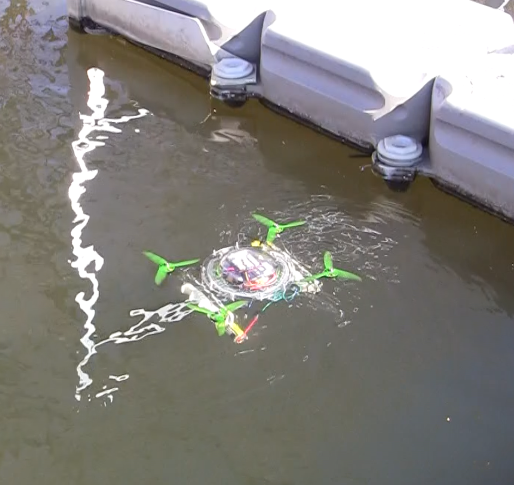
\includegraphics[trim=0 50 0 70,clip,width=\textwidth]{images/omnibot/omnibot_river_dock_small.png}
     \caption{Water operation.}
     \label{fig:omnibot_river}
   \end{subfigure}
   \begin{subfigure}[t]{0.38\textwidth}
     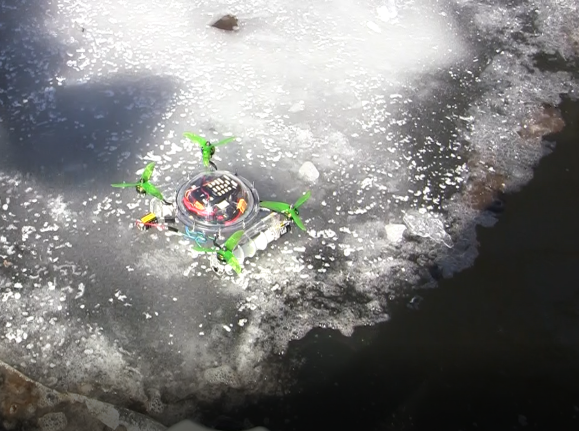
\includegraphics[trim=0 50 0 50,clip,width=\textwidth]{images/omnibot/omnibot_ice_2_small.png}
     \caption{Resting on floating ice.}
     \label{fig:omnibot_ice}
   \end{subfigure}
   \begin{subfigure}[t]{0.30\textwidth}
     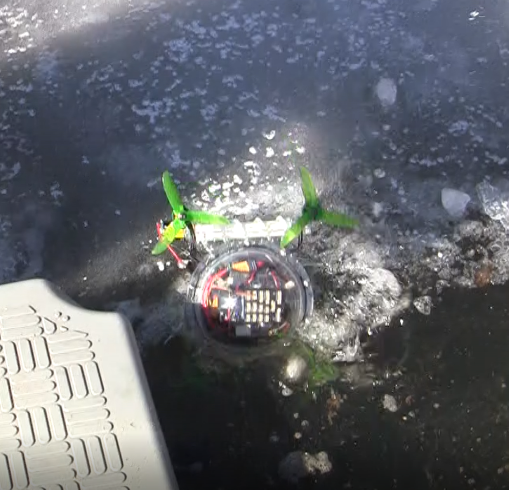
\includegraphics[trim=0 0 0 120,clip,width=\textwidth]{images/omnibot/omnibot_ice_water_transition_small.png}
     \caption{Ice to water transition.}
     \label{fig:omnibot_ice_water}
   \end{subfigure}
   \caption{Outdoor Omnibot prototype testing on the Mississippi River.}
   \label{fig:omnibot_outdoor_test}
\end{figure*}

After indoor testing of the Omnibot in each individual environment, testing in a real-world setting at the docks of the University of Minnesota Boathouse on the Mississippi River was planned. At the time of the experiments river ice was common around the dock and there was a section of floating ice trapped next to the docks that served as a convenient platform for launching the Omnibot (Figure~\ref{fig:omnibot_ice}).  

The outdoor experiments consisted primarily of water navigation, locomotion on ice, and the transition from the floating ice shelf into the water to verify functionality. The first experiment was of the screwdrive for water locomotion (Figure~\ref{fig:omnibot_river}). Next the robot was manually placed on the floating ice and maneuvered in a circle. Lastly, a land to water transition was carried out by driving the robot off the ice and into the cold Mississippi water (Figure ~\ref{fig:omnibot_ice_water}).

The experiments were successful in that they functioned as expected, with the screwdrive system successfully moving the robot in the water, on the ice, and during the launch. To note was the forward traction of the screwdrive on the impenetrable ice, this is though to be due to the low friction between the ice and the screws allowing the robot to ``skate'' on ice.  

%The outdoor experiments were carried out at approximately 27 degrees Farenheit, although the water temperature was not measured, it was as cold, if not colder. This was significant due to the elastomeric nature of the seals, which can shrink and become brittle under low temperatures. 

\subsubsection{Proposed Work}
\label{omnibot_proposed}

We propose creating a novel platform capable of navigating water, land, and air in order to expand the available types of environments that can be monitored and giving unprecedented ability to use the best locomotion type to overcome obstacles and unforeseen circumstances. The platform would be developed to demonstrate:

\begin{itemize}
  \item Operation and seamless transition between all domains.
  \item Integration of sensor payloads for environment monitoring.
  \item Characterization of energy expenditure in each enviroment.
\end{itemize}



%Omnibot background ------------------------------------------------------------------------------------
%On the other hand, there have also emerged a handful of systems that can perform tasks in two or three kinds of regions, making them especially suitable to carry out more complex tasks in varying or changing environments. However, none of them could cover all four common kinds of territories including land, air, water surface and under water.

%Nowadays, various kinds of autonomous systems are being intensively developed and deployed to numerous civil and military application areas. According to their active regions, they can be divided into two groups, specialized robotic platforms including UGVs, UAVs, USVs and UUVs, and multi-purpose ones, which are composed of vehicles that can cover more than one fields. 

%UGVs operate while in contact with the viground. Therefore, they can gather information at a much higher resolution than UAVs. Nonetheless, UGVs are usually much slower in terms speed and efficiency. Furthermore, they are constrained by whatever obstacles may be present in their environment. 

%USVs can float in the water, monitor the water surface, and even look into the water in a limited fashion. They are valuable for oceanography due to its low cost and flexibility compared with other means.

%UUVs are targeted for underwater applications, including seabed surveillance, fish and current monitoring, etc. Nonetheless, they may suffer from communication and power supply issues. Typically these platforms are either tethered or prohibitively expensive due to the sensors required for localization in a GPS-denied environment. Furthermore, these expensive platforms generally require a larger vessel to transport, deploy, and pick up, adding to overall costs. 

%On the other hand, some types of multi-purpose systems have also been proposed, most of which can enter two kinds of regions while few could cover three modes.

%As a matter of fact, robots that can cover two kinds of regions are not rare. One case in point is that of the hybrid air-water microrobot from Chen et al. \cite{Chen2017} which weighs 175 milligrams. This aerial-aquatic microrobot is capable of flapping its wings to propel itself through air and water. The water to air transition is not simple as it has to overcome significant surface force. Moreover, it has to overcome limitations of flapping wing motion to take off from the surface. The microrobot achieves this by igniting a small chemical reaction to propel itself away from the surface of the water.

%Another example is the AQUA \cite{Dudek2007c}, which is a bi-modal amphibious robot that employs flipper-like legs to move from land and into the water. It uses six appendages to propel itself in the water while using a cockroach-like gait when walking on land. The legs are compliant which serves to provide additional terrainability to the robot. 

%On the miniature robotics side of the spectrum, the Aquapod \cite{Dhull2012} is an amphibious robot that moves around by effectuation tumbles on land and using a buoyancy control unit (BCU) in the column of water. 

%Comparatively, few platforms can navigate through more than two regions. The multi-field universal wheel for the air-land vehicle (MUWA) \cite{Kawasaki2013} turns out to be the only example in this category that we could find. As we can see from Figure \ref{fig:muwa}, the MUWA can fly in the air, float on the water and rotate on the land at an arbitrary angle using a specially designed control algorithm. 

%\cite{Siddall2014} AquaMAV
%\cite{Kossett2013} Hybrid 
%\cite{Mintchev} very similar to Alex's hybrid
%\cite{Alzubi2018} Loon Copter 

%Aquatic–aerial unmanned vehicles recently became the focus of many researchers due to their various possible applications. Achieving a fully operational vehicle that is capable of aerial, water- surface, and underwater operations is a significant challenge considering the vehicle's air–water– air transition, propulsion system, and stability underwater.We present in this paper an unconven- tional unmanned hybrid aquatic–aerial quadcopter with active buoyancy control that is capable of aerial flight and water-surface operation, as well as subaquatic diving. We report on the first successful prototype of the vehicle, named the Loon Copter, to provide initial evaluation results of its performance in both mediums. The Loon Copter uses a single set of motors and propellers for both air and underwater maneuvering. It utilizes a ballast system to control vehicle buoyancy and depth underwater, as well as to perform seamless air-to-water and water-to-air transitions. A closed loop control algorithm is utilized for the vehicle's aerial and water-surface stability and maneuver, whereas an open loop control algorithm is used for underwater maneuver. The experi- mental results show a fully operational prototype with six degrees of freedom underwater, stable flight, operation capabilities onwater surface, and agile maneuvering underwater.

%Omnibot background ------------------------------------------------------------------------------------






%intro?:
%When designing a robot around an intended application or class of applications, there are a number of cross-corelated factors that should be taken into account, such as weight, payload, sensors, type of environment, battery size, actuator size, shape of the external structure, type of environment, chemical compatibility, among others that will determine the efficacy of the robot in carrying out the mission. For example, a small inexpensive robot, would not have the ability to carry large sensors or actuators. 

%TODO: move to multi-environments robots. 
%The Multi-field Universal Wheel for Air-land Vehicle (MUWA) \cite{Kawasaki2013}, Fig~\ref{fig:muwa}, almost achieves this feat in that it operates on land, air, and on the \emph{surface} of a body of water. Consisting of a traditional quad-rotor layout, it is surrounded by a dual styrofoam rings on its periphery. The MUWA uses four variable pitch propellers to control thrust and manuever in the air. When on land, it is able to use this differential thrust to stand itself up on its side and roll on the outer rings as a mono-wheel. These outer rings are positively buoyant and enable the robot to float on the surface of the water and the actuators provide ability to move about in a limited fashion. That being said, Kawasaki et al. did not design the robot to be capable of underwater operation.  

%With the Omnibot, the end goal is a platform that can perform environmental monitoring in all three domains, using flight to transport itself quickly between locations and leveraging its unique capabilities to optimally perform the task at hand. This platform would ideally use a multi-rotor design for flight, a buoyancy control unit to alter its density, a waterproof hull to travel through and in water, and a dual screw system to move about on land and in water. 


%Operation in the three domains is more than the combination of parts as constraints for one domain are often at odds with another domain's contraints. Some contraint conflicts are obvious, such as the minimum necessary weight to enable land and water operation versus flight performance. Other constraints, such as neutral buoyancy, are more nuanced, since weight minimization is favorable for flight but ballast weight may be needed to match the platform's displaced volume. 

%In the case of the MUWA robot, its outer flotation rings keep the robot positively buoyant preventing the robot from going underwater. That being said, even if that were not the case, the electronics would have to be not only water resistant, but waterproof. This is generally stated in terms of ingress protection IP Code, where IP61 would be considered resistant to light water, like rain, and IP67 would mean suitable for conditions of immersion at up to 1 meter. 


%Leveraging a new propulsion method for land and water locomotion in conjunction with  quad and octo-rotor designs for flight, the Amphibot will utilize a buoyancy control unit to alter its density and its waterproof hull to travel through and in water, over land, and to fly through the air. 

%A removable payload “disc” around its periphery will be used to extend the capabilities of the robot in various important ways. Its will reduce frictional losses while moving through air and land. Different sensor suites will be mounted on the disk in such a way to allow easy deployment of many Amphibots with different sensor payloads. 

%The Amphibot will utilize a NVIDIA Jetson TX2 board to simultaneously gather sensor data from six cameras: downward-facing, upward-facing, and four around the periphery of the robot. This array of cameras will allow omnidirectional proprioception. Leading to interesting opportunities for a number of activities such as: crop monitoring on land and air, lake health evaluation from the air, surface, and in the water, search and rescue missions, etc. 


%The Aquapod's strengths can be seen in that it leverages its amphibious nature to navigate and perform measurements in both land and water environments.  Compared to the terrestrial Adelopod, it greatly expanded the nature and type of sensing that could now be undertaken. Terrains that were once inaccessible, such as mud, puddles, and snow, were now traversable and environmental monitoring could be undertaken on environments like lakes and streams. 

%$$ \rho_{omnibot} = (mass_{omnibot}+mass_{bladder})/volume_{omnibot} $$ 

%When the mass of the ingested media is enough to alter the OmniBot's density above that of the media it is contained in, it sinks. Reversing this process leads to the robot floating upwards towards the surface. 

%$$ \rho_{omnibot} > \rho_{water} $$
%$$ \frac{\rho_{omnibot}}{\rho_{water} } > 1 $$
%$$ \rho_{water} = 1000 \frac{kg}{m^3} = 1 \frac{g}{cm^3} $$ 

